\documentclass{scrartcl}

% packages
\usepackage[utf8]{inputenc}
\usepackage{tikz}
    \usetikzlibrary{positioning}
\usepackage[american, cute inductors, RPvoltages]{circuitikz}

\begin{document}

    \begin{figure}[ht!]
      \centering
        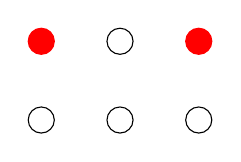
\begin{tikzpicture}
            [
                armadura/.style={circle, draw=red, fill=red},
                serie/.style={circle, draw},
                paralelo/.style={circle,draw},
            ]
            % armadura
            \node[armadura] (A1) at (0,0) {};
            \node[armadura] (A2) at (2,0) {};
            % enrolamento série
            \node[serie] (serie1) at (1,0) {};
            \node[serie] (serie2) at (1,-1) {};
            % enrolamento paralelo
            \node[paralelo] (paralelo1) at (0,-1) {};
            \node[paralelo] (paralelo2) at (2,-1) {};
        \end{tikzpicture}
      \caption{Terminais do gerador de corrente contínua. Destacados os
        terminais de armadura. Os terminais abaixo dos terminais de armadura
        são os terminais de enrolamento paralelo}
      \label{fig:terminais-gerador}
    \end{figure}

    \begin{figure}[ht!]
      \centering
        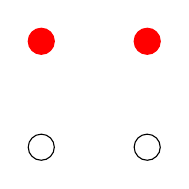
\begin{tikzpicture}
            [
                armadura/.style={circle, draw=red, fill=red},
                serie/.style={circle, draw},
                paralelo/.style={circle,draw},
            ]
            %obs: \usetikzlibrary{positioning}
            \node[armadura] (a1) {};
            \node[armadura] (a2) [right=of a1] {};
            \node[paralelo] (p1) [below=of a1] {};
            \node[paralelo] (p2) [below=of a2] {};
        \end{tikzpicture}
        \caption{Representação somente dos terminais de armadura e do
        enrolamento paralelo. 
        (Trying to use relative placement. How to add nodes
        betweeen? Not so simple)}
      \label{fig:terminais-gerador}
    \end{figure}


    \begin{figure}[ht!]
      \centering
      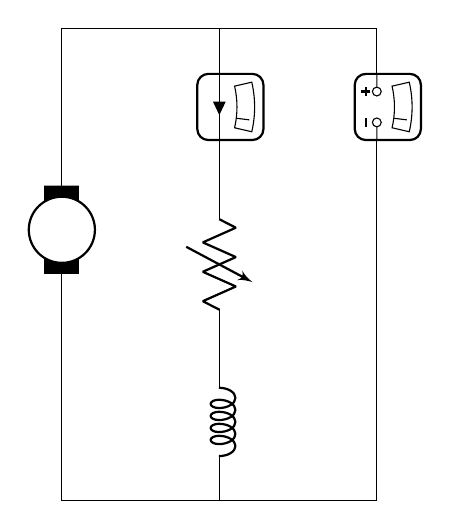
\begin{tikzpicture}
          \draw (0,0) node[elmech](gen){};
          \draw (gen.north) -- ++(0,2) -- ++(2,0) coordinate (a1); 
          \draw (a1) to[qiprobe] ++(0,-2) to[vR] ++(0,-2) to[L] ++(0,-2) 
            coordinate (f2);
          \draw (f2)  -| (gen.south);
          % voltimetro
          \draw (a1) -- ++(2,0) to[qvprobe]++(0,-2) |- (f2);
      \end{tikzpicture}
    \end{figure}

\end{document}
